% Chapter 2
\documentclass[../main.tex]{subfiles}
\begin{document}

The model we have created applies methods well-known in the field of statistics, however applying these methods to our model brings unique issues/decisions. In this chapter we will discuss these complications and explain and justify the decisions we make going forward. 

%% ISI distribution section.   
\section{ISI Distribution}

% Intro of the importance of the ISI distribution. What it involves and what it can inform us on. Why we care.
In this section we discuss the importance of the inter-spike interval (ISI) distribution. In Chapter 2 --- page { \color{red} XX} --- we gave an example whereby we created a ISI distribution by extending the one dimension Gamma $(\gamma, \gamma)$ distribution. The extension is performed by applying a time-rescaling method via the intensity function $x(t)$ which accounts for the time-dependence of \ce{Ca^2+} spiking. A natural question is why did we choose the one dimension Gamma distribution and is the choice of distribution important? 

To begin, let us first consider the case of stationary \ce{Ca^2+} spikes --- by this we mean spikes that depends only on the time since the last spike and not the time of the experiment. Thus the ISI distribution can be modelled as a function of the time $s$ since the last spike, whose domain is $(0,\infty)$. We can choose to model the ISI distribution $\psi (s)$ as common probability distribution such as: an Exponential distribution 
$$ \psi (s | \alpha ) = e^{-\alpha s}$$
  a Gamma distribution
   $$ \psi(s| \alpha, \beta ) = e^{-\alpha(t_2-t_1)}$$,
 or a Weibull distribution
   $$ \psi(s | \lambda, k ) = e^{-\alpha}$$
   
 where $\{ \alpha\}$, $\{\alpha, \beta\}$ and $\{\lambda , k\}$ the ISI parameters for distribution respectively. Each distribution, can be justified as a model for the ISI distribution. For example, if we believed spikes occur independently then the exponential distribution is suitable. 
% Add Gamma just and Inv Gauss just. 

To find which of the models best describes a \ce{Ca^2+} spike sequence we first convert the spike sequence into a sequence of $M$ ISI times $\{T_i\}_{i=1}^M$. Then to fit each model $\psi(s|\theta)$ with $\theta$ the probability distributions parameter/s we calculate the MAP estimator by 
$$\hat \theta  = \mathrm{arg max} \left\{ \prod ^M_{i=1} \psi(T_i | \theta ) \right\}$$.

%Example using Ca spike sequence. 
We consider a spike sequence from a HEK293 cell stimulated 



%Summary of the stationary case. 
The above shows that the choice of ISI distribution parameterisation is important, as we find different distributions are more suitable than others. 
At this stage, one could argue to use a non-parameteric method to estimate the ISI distribution. This would indeed be a more flexible framework since the ISI distribution would not be limited to the shape of the chosen probability distribution. 
However, it is important to note although we may find that one probability distribution best describes the \ce{Ca^2+} spikes, there may exist a better untested model. 
In this setting another option would be to use histogramming, kernel densities, or non-parametric methods to infer the ISI distribution. 
 

%Back to our model.
Returning to our model, we can generalise any probability distribution on $(0,\infty)$ to create a non-stationary ISI distribution. To generalise the distribution $\psi(s|\theta)$ we rescale time via the positive intensity function $x(t)$. In this new time 
$$ p(s,t |x,\theta) = x(t)\psi (\int^t_s x(u)du|\theta) $$.

Thus, by applying the transformation we create the (inhomogenous) Gamma

$$
 p(y_i, y_{i-1}| x, \alpha, \beta) =  \frac{\beta x(y_i)}{\Gamma ( \alpha )} \big[ \beta X(y_{i-1} , y_i ) \big]^{\alpha -1} \exp( - \beta X(y_{i-1} , y_i )  ),
$$
 the inhomogenous


% Non identifiability. 


In our model we consider time-dependent \ce{Ca^2+} spiking. In practice, this is done by extending the concept of modelling the ISI distribution with a known probability distribution via the time-rescaling theorem. We begin by choosing a probability distribution $p_{\mathrm{stat}}$ on $(0,\infty)$ with parameter/s $\theta$. We then introduce the intensity function $x(t)$ defined on the experiment time $[0,T]$. By rescaling the ISI 

Recall, in our model we are considering time-dependent \ce{Ca^2+} spiking. Thus we generalise the ISI distribution via the time-rescaling theorem. Recall from Chapter 2 we begin by choosing a probability distribution $p_{\mathrm{orig}}(t_1,t_2 | \theta)$. 


To stress the importance of the choice of ISI distribution suppose we have given a spike sequence containing 35 spikes over 2800s. Assuming the spiking rate is constant we expect the mean time between spikes to be 80s. Suppose we chose the an exponential as the ISI distribution. 
  \begin{figure}[t]
   \hrulefill
   \begin{center} 
    \subfloat{{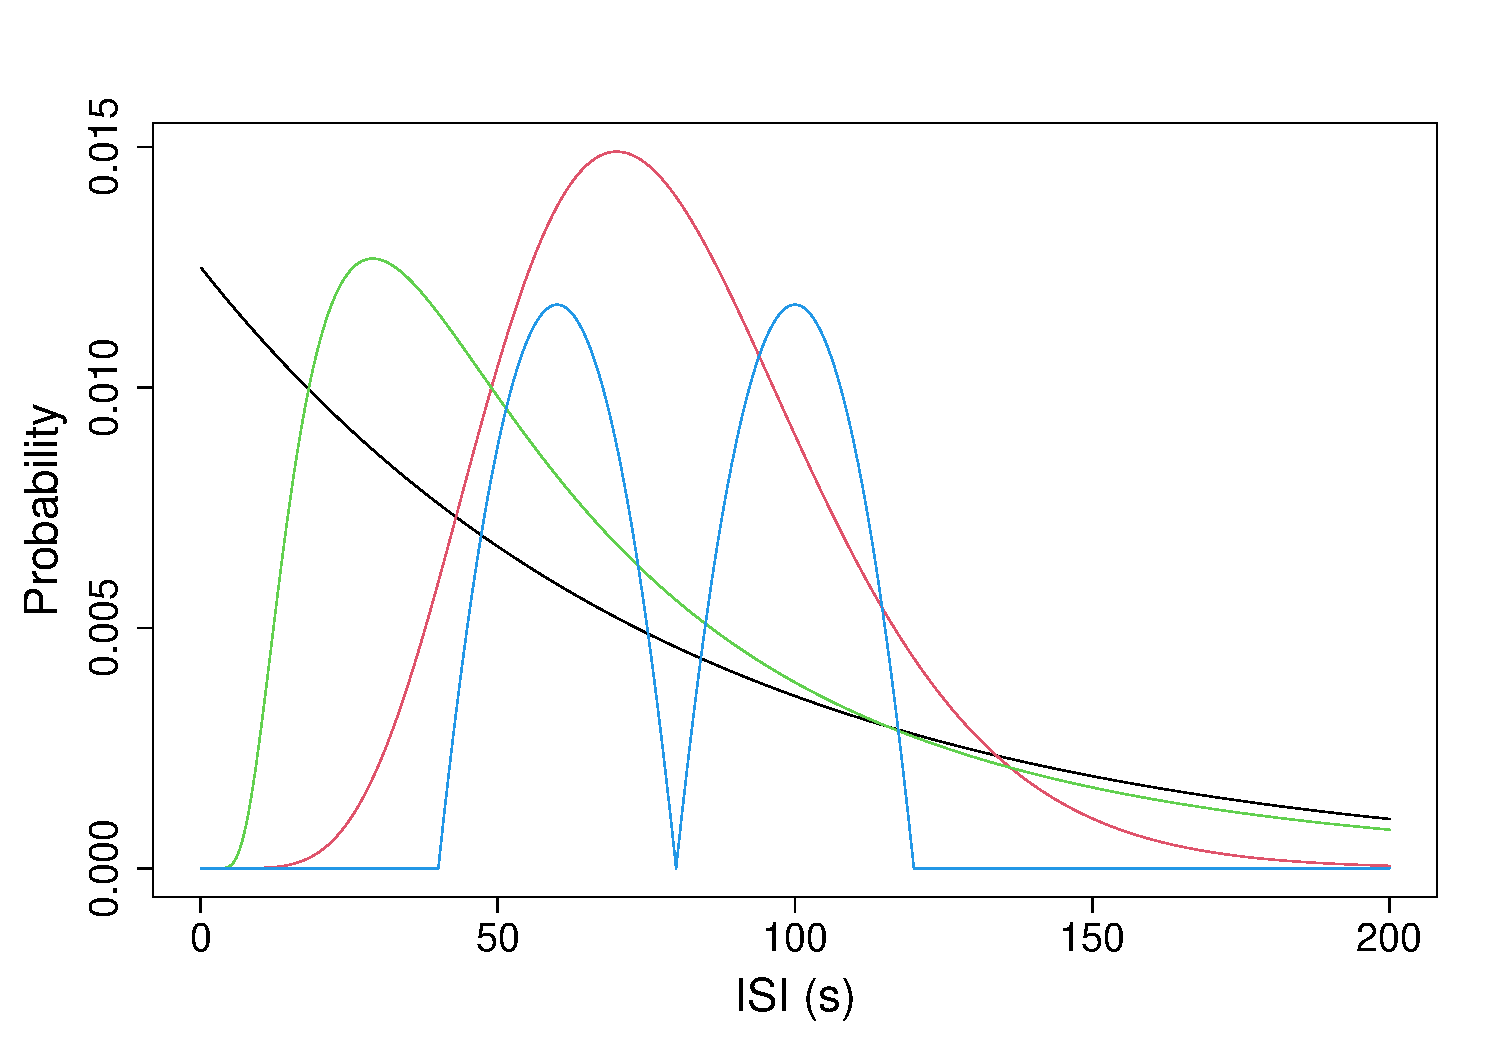
\includegraphics[width=0.8 \linewidth]{ExampleISI} }}
    \end{center}     
    \caption{Example ISI distributions.   }
    \label{fig:ExampleISI}
    \hrulefill
    \end{figure}

In figure \ref{fig:ExampleISI} we 

% Summary of how we generalise to allow for non-stationary spikes. With justification why we want to do this. 
In the above example the we assumed that the spiking rate is constant, however our model is based on the assumption that the spiking rate varies over time. Thus, figure \ref{fig:ExampleISI} is a snapshot of how the ISI distribution looks at a single moment in time. 
To model the time-heterogeneity we transform the original probability distribution via the time-rescaling theorem, as described in Chapter 2. To summarise this approach we begin fixed distribution $p$ with parameters $\theta$ to describe the ISI distribution in the stationary setting. To generalise for non-stationary spikes we apply the transform to this distribution and obtain the inhomogeneous ISI distribution which depends on the parameters $\{\theta, x\}$, where $x$ is the intensity function. 

\begin{align} \label{eq:5}
g(z_i,z_{i+1} | x) =& \frac{dz}{dt} \bigg\rvert_{y_{i+1}} p(z_i, z_{i+1}),  \\
=& x(y_{i+1}) p(z_i, z_{i+1}). \label{eq:5b}
\end{align}

----%Example of the weibull dist. 


% Consider previous results and which models were considered. Pros and cons. 

% How can we extend to consider more ISI distributions.
Our aim is to extend the number of ISI distributions used to model \ce{Ca^2+} spikes, which the intention of confirming that the Gamma distributions performs best or finding a distribution that better describes \ce{Ca^2+} spikes. 

% Option 1 include more base probability dists. Why these distributions? 
We first extend the number of ISI distributions considered by also using a Weibull and Log Normal distribution. The motivation behind these distributions are ... 
 
% Option 2. Note that the previous results only considered 1-D dists of G and IG. Can we generalise? 
The second approach is by generalising the current distributions. Consider the ISI distributions used by Titunaite et al, these are inhomogeneous versions of Gamma$(\gamma, \gamma)$ and Inverse Gaussian $(\alpha,1)$ distributions. Hence they are inhomogeneous versions of one-parameter distributions. Thus, a natural question is why did they choose one-parameter version of these distributions and can we generalise these distributions to their two-parameter counterparts?  

% Non identifiability of generalised models. 
We begin by considering the Gamma distribution 
$$ 100$$ 
transforming via the time-rescaling theorem gives the inhomogeneous two-parameter Gamma distribution as 
\begin{equation*}
 p(y_i, y_{i-1}| \alpha, \beta, x(t)) =  \frac{\beta x(y_i)}{\Gamma ( \alpha )} \big[ \beta X(y_{i-1} , y_i ) \big]^{\alpha -1} \exp( - \beta X(y_{i-1} , y_i )  ),
 \end{equation*}
 
 One way to visualise this, is that the intensity function replaces one of the parameters of the original distribution. 

% Choosing the version of each model. Why? 
	
%Figure of comparing histograms with different parameterisations. 
  \begin{figure}[t]
   \hrulefill
   \begin{center} 
    \subfloat{{\includegraphics[width=0.8 \linewidth]{CompareHist} }}
    \end{center}     
    \caption{Histograms comparing the intensity to histograms of 1000 simulated spike sequences. The light and dark histograms correspond to simulating spikes with ISI distributions Gamma(1.8,1.8) and Gamma(3.6,1.8) respectively.  }
    \label{fig:CompareHist}
    \hrulefill
    \end{figure}
    
% Possible further extensions. Include refractory explicitly. 













The ISI distribution is an important piece of the \ce{Ca^2+} spiking mechanism. In fact, if we assumed the spiking rate was stationary the ISI distribution would fully describe the \ce{Ca^2+} spikes. 

It is important to note that apriori we have little idea what the ISI distribution will look like. 








%An integral part of our model is the ISI distribution. The ISI distribution informs characterises how spike times are related to each other etc. A priori there is no information on what ISI distribution will best describe the \ce{Ca^2+} spikes. Any probability distribution on $[0,\infty )$ could be used to describe the ISI distribution. 
In our methodology we begin by choosing a probability distribution $p$ on $[0,\infty )$ --- such as a exponential or Gamma distribution. Then to allow for heterogeneity we apply the time rescaling theorem to generate a probability model dependent on the intensity function $x(t)$ and probability distribution $p$ with parameters $\theta$. In Chapter 2 we described how to infer the model parameters when the chosen probability distribution was a Gamma distribution. However, there is no prior information suggesting that the Gamma is the best distribution to use. 


%Discussion of previously used ISI distributions. 
However, Titunate et al \cite{} have tested 3 probability distribution to HEK293 cells stimulated with Carbohol. The ISI distributions they tested were the 
%In Chapter 2 we assumed that the ISI distribution follows an inhomogeneous gamma distribution as detailed in equation ---. This is the model that was found to perform best by Titulane et al \cite{} when applying similar methods to HEK293 cells stimulated with Carbohol. In their paper they tested three potential ISI distributions, which they named the
 (inhomogeneous) Poisson 
$$
p(y_i,y_{i-1} | x) = x(y_i) e^{-X(y_i,y_{i-1})} ,
$$

the (inhomogeneous) Gamma

$$
p(y_i,y_{i-1} | x,\gamma) = \frac{\gamma x(y_i)}{\Gamma(\gamma)}\left[\gamma X(y_i,y_{i-1}) \right]^{\gamma -1} e^{-\gamma X(y_i,y_{i-1})},
$$

and the (inhomogeneous) Inverse Gaussian

$$
p(y_i,y_{i-1} | x,\alpha) = \frac{x(y_i)}{\sqrt{2 \pi X(y_i,y_{i-1})^3}} \exp \left\{ -\frac{\left( X(y_i,y_{i-1}) - \alpha \right)^2}{2 \alpha^2 X(y_i,y_{i-1}) } \right\}.
$$
The inhomogeneous Poisson is the simplest inhomogeneous point process, based on an exponential ISI probability distribution. Titunate et al found that the inhomogeneous Gamma distribution preformed best out these ISI distributions by comparing QQ and KS plots --- see chapter 5? for a discussion on how these methods compare ISI distributions. 

Clearly, this is not an exhaustive list of all potential probability distributions that can explain the ISI distribution. Thus, it is possible that a different distribution may describe the \ce{Ca^2+} spikes equally well or better than the Gamma ISI distribution above. 

Recall when describing the model we begin by first considering a homogeneous process. We choose the probability distribution $p$ on $[0,\infty)$, with parameters $\theta$ to describe the ISI distribution. Then we extend to a time-dependent model by applying the time-rescaling theorem where in the new time  
 
The first distribution is called the inhomogenesous Poisson because the exponential distribution leads to the definition of a Poisson process. This ISI distribution    These distributions were chosen because ... . However, this is clearly not a list of all possible distributions, and it is possible that another non-tested distribution would give a better fit. Thus, we will extend the number of ISI distributions to be considered to include a Log Normal distribution and a Weibull distribution. We want to consider these distributions because ... . 

%Extend by generalising distributions

% Decide on the parameterisation we want.
Above we have seen that 

    
Notice that the IG and IIG distributions are generalisations of one-parameter Gamma and Inverse Gaussian distributions, namely Gamma $(\gamma, \gamma)$ and InverseGaussian$(\alpha,1)$.

By the introduction of the intensity function we can see that the above distributions are generalisations of one-parameter Gamma and Inverse Gaussian distributions, namely Gamma$(\gamma, \gamma)$ and InverseGaussian$(-,-)$. A natural question would be to ask whether we can generalise further and allow for the distributions two-parameter versions, such as the Gamma$(\alpha, \beta)$. However, by generalising the ISI distribution we create non-identifiability issues, where by scaling the ISI parameters with the intensity function we 
 
\subsection{Non-Identifiability issues with two parameter ISI distributions} 
To begin we will consider the Gamma distribution. Thus suppose the ISI distribution is defined by

\begin{equation}
 p(y_i, y_{i-1}| x, \alpha \beta) =  \frac{\beta x(y_i)}{\Gamma ( \alpha )} \big[ \beta X(y_{i-1} , y_i ) \big]^{\alpha -1} \exp( - \beta X(y_{i-1} , y_i )  ),
 \end{equation}
 
 where 
  \begin{equation}
X(s,t) = \int^{t}_{s} x(u) du , \qquad \text{for any } s,t \in [0,T].
\end{equation}


 
\subsection{Choosing one-parameter ISI distributions}
Thus, we for each of the generalised two-parameter ISI distributions we need to choose a parameterisation to remove the non-identifiability issues. 

Thus, the ISI distributions we will consider are the following:

%GAMMA
\subsection{Gamma distribution}
Throughout we have assumed that the Gamma ISI distribution is as follows 
\begin{equation}
 p(y_i, y_{i-1}) =  \frac{\gamma x(y_i)}{\Gamma ( \gamma )} \big[ \gamma X(y_{i-1} , y_i ) \big]^{\gamma -1} \exp( - \gamma X(y_{i-1} , y_i )  ).
 \end{equation}
 
 Which one can see a generalisation of a Gamma$(\gamma,\gamma)$. We have used this distribution because it was used in \cite{}. However, can we generalise further and consider a Gamma$(\alpha,\beta)$ ISI distribution? The answer is no. This is because the parameters $x$ and $\beta$ are non-identifiable.  \\
 
{\color{blue}
Suppose our ISI interval is given by the following $(\alpha, \beta )$ Gamma distribution. 

\begin{equation}
 p(y_i, y_{i-1}) =  \frac{\beta x(y_i)}{\Gamma ( \alpha )} \big[ \beta X(y_{i-1} , y_i ) \big]^{\alpha -1} \exp( - \beta X(y_{i-1} , y_i )  ),
 \end{equation}
 
 where 
  \begin{equation}
X(s,t) = \int^{t}_{s} x(u) du , \qquad \text{for any } s,t \in [0,T].
\end{equation}
 
 Now we will show that this is equivalent to a $(\gamma, \gamma)$ Gamma distribution by scaling the intensity function.\\
 
 Let $\gamma = \alpha$ and $\kappa = \frac{\beta}{\alpha}$, thus giving $\beta = \gamma \kappa$. Substitute into (2) gives
 
 \begin{equation}
 p(y_i, y_{i-1}) =  \frac{\gamma \kappa x(y_i)}{\Gamma ( \gamma )} \big[ \gamma \kappa X(y_{i-1} , y_i ) \big]^{\gamma -1} \exp( - \gamma \kappa X(y_{i-1} , y_i )  ).
 \end{equation}
 
 Now define new intensity function by $\tilde x = \kappa x$, hence giving
 
   \begin{equation}
\tilde X(s,t) = \int^{t}_{s} \tilde x(u) du = \int^{t}_{s} \kappa x(u) du =  \kappa X(s,t)  , \qquad \text{for any } s,t \in [0,T].
\end{equation}

Put this into (3) gives
 \begin{equation}
 p(y_i, y_{i-1}) =  \frac{\gamma  \tilde x(y_i)}{\Gamma ( \gamma )} \big[ \gamma \tilde X(y_{i-1} , y_i ) \big]^{\gamma -1} \exp( - \gamma \tilde X(y_{i-1} , y_i )  ),
 \end{equation}
 
 which we see is a $(\gamma, \gamma)$ Gamma distribution. \\
 
 Hence, where we have introduced a two-variable Gamma distribution we cannot retrieve initial choices of variables. I.e $\beta$ is replaced as a variable by the intensity function. The choice of having $\alpha = \beta$ is a sensible choice as this allows the expected number of spikes to not depend on the ISI parameters and only depends on $x$.
 }
 
 %Inverse Gaussian
 \subsection{Inverse Gaussian distribution}
 Similarly we have not considered the full generalised Inverse Gaussian ISI distribution
 \begin{equation}
 p(y_i, y_{i-1}) =  x(y_i) \bigg( \frac{\lambda}{2\pi X(y_{i-1} , y_i )^3} \bigg)^{0.5} \exp \bigg[-\frac{\lambda(X(y_{i-1} , y_i )-\mu)^2}{2 \mu ^2 X(y_{i-1} , y_i )} \bigg].
 \end{equation}
 
 However, we again get non-identifiable variables, in this case if we multiple all the parameters by a constant we get an identical distribution. \\
 
 {\color{blue}
 Suppose we have an Inverse Gaussian ISI distribution with parameters $(\lambda,\mu)$ and intensity function $x$. We want to show this is identical to an IG$((k\lambda,k\mu))$ with intensity $kx$ for any constant $k$. Firstly, note that the constant comes out the front of of the integral of the intensity function. 
 
    \begin{equation}
 \int^{t}_{s} \kappa x(u) du = \kappa \int^{t}_{s} x(u) du = \kappa X(s,t)  , \qquad \text{for any } s,t \in [0,T].
\end{equation}

Hence, we get
  \begin{align}
 p(y_i, y_{i-1}|kx,k\lambda,k\mu) &=  kx(y_i) \bigg( \frac{k\lambda}{2\pi (kX(y_{i-1} , y_i ))^3} \bigg)^{\frac{1}{2}} \exp \bigg[-\frac{k\lambda(kX(y_{i-1} , y_i )-k\mu)^2}{2 (k\mu) ^2 kX(y_{i-1} , y_i )} \bigg],\\
 &=  kx(y_i) \bigg( \frac{1}{k^2}\frac{\lambda}{2\pi X(y_{i-1} , y_i )^3} \bigg)^{\frac{1}{2}} \exp \bigg[-\frac{k\lambda(k(X(y_{i-1} , y_i )-\mu))^2}{2 k^3\mu ^2 X(y_{i-1} , y_i )} \bigg],\\
  &=  \frac{k}{k}x(y_i) \bigg(\frac{\lambda}{2\pi X(y_{i-1} , y_i )^3} \bigg)^{\frac{1}{2}} \exp \bigg[-\frac{k^3}{k^3}\frac{\lambda(X(y_{i-1} , y_i )-\mu)^2}{2\mu ^2 X(y_{i-1} , y_i )} \bigg],\\
 &=  x(y_i) \bigg( \frac{\lambda}{2\pi X(y_{i-1} , y_i )^3} \bigg)^{\frac{1}{2}} \exp \bigg[-\frac{\lambda(X(y_{i-1} , y_i )-\mu)^2}{2 \mu ^2 X(y_{i-1} , y_i )} \bigg],\\
 &= p(y_i, y_{i-1}|x,\lambda,\mu) \qquad \qquad \text{as required.}
 \end{align}
 }
 
 %Log Normal
 \subsection{Log Normal distribution}
 Next we shall consider the full Log Normal distribution
 
 \begin{equation}
 p(y_i, y_{i-1}) = \frac{x(y_i)}{X(y_{i-1} , y_i ) \sigma \sqrt{2 \pi}} \exp \left\{ -\frac{(\log X(y_{i-1} , y_i ) - \mu)^2}{2\sigma^2} \right\}
 \end{equation}
 
 However as in the above two cases we get non-identifiable variables. In this case, if we multiply the intensity by a factor of $\kappa$ this is identical to subtracting $\log \kappa$ to $\mu$.\\
  {\color{blue}
   Suppose we have an Log Normal ISI distribution with parameters $(\mu,\sigma)$ and intensity function $\kappa x$. We want to show this is identical to an LN$((\mu + \log \kappa,\sigma))$ with intensity $\kappa x$ for any constant $\kappa$.
   
     \begin{align}
 p(y_i, y_{i-1}|\kappa x,\mu,\sigma) &= \frac{\kappa x(y_i)}{\kappa  X(y_{i-1} , y_i ) \sigma \sqrt{2 \pi}} \exp \left\{ -\frac{(\log\kappa  X(y_{i-1} , y_i ) - \mu)^2}{2\sigma^2} \right\},\\
 &=   \frac{ x(y_i)}{  X(y_{i-1} , y_i ) \sigma \sqrt{2 \pi}} \exp \left\{ -\frac{(\log\ X(y_{i-1} , y_i ) + \log \kappa - \mu)^2}{2\sigma^2} \right\}\\
 &=   \frac{ x(y_i)}{  X(y_{i-1} , y_i ) \sigma \sqrt{2 \pi}} \exp \left\{ -\frac{(\log\ X(y_{i-1} , y_i )  - (\mu - \log \kappa))^2}{2\sigma^2} \right\}\\
 &= p(y_i, y_{i-1}|x,\mu - \log \kappa,\sigma) \qquad \qquad \text{as required.}
 \end{align}
  }
  
   %Weibull
 \subsection{Weibull distribution}
 Next we shall consider the Weibull distribution
 
 \begin{equation}
 p(y_i, y_{i-1}|k,\lambda) = \frac{x(y_i)k}{\lambda} \left( \frac{X(y_{i-1} , y_i )}{\lambda} \right)^{k-1} \exp \left\{ -\left( \frac{X(y_{i-1} , y_i )}{\lambda} \right)^k \right\}
 \end{equation}
 
 However again we get non-identifiable variables. In this case, if we multiply the intensity by a factor of $m$ this is identical to dividing $\lambda$ by $m$. \\
  {\color{blue}
   Suppose we have an Weibull ISI distribution with parameters $(k,\lambda)$ and intensity function $m x$. We want to show this is identical to an Weibull$(k,\frac{\lambda}{m})$ with intensity $x$ for any constant $m$.
   
     \begin{align}
 p(y_i, y_{i-1}|mx, k, \lambda) &= \frac{mx(y_i)k}{\lambda} \left( \frac{mX(y_{i-1} , y_i )}{\lambda} \right)^{k-1} \exp \left\{ -\left( \frac{mX(y_{i-1} , y_i )}{\lambda} \right)^k \right\} \\
 &=\frac{x(y_i)k}{\lambda/m} \left( \frac{X(y_{i-1} , y_i )}{\lambda/m} \right)^{k-1} \exp \left\{ -\left( \frac{X(y_{i-1} , y_i )}{\lambda/m} \right)^k \right\} \\ 
 &= p(y_i, y_{i-1}|x,k, \lambda/m) \qquad \qquad \text{as required.}
 \end{align}
  }
 
% \section{Why we choose the ISI distribution to have mean 1}
% Throughout we have defined $x(t)$ to be the intensity function, this means that at any time $t$ $x(t)$ is the rate of spikes. Hence $X(t , s)$ is the expected number of spikes in the interval $[t,s]$. Suppose we choose the ISI distribution to follow the probability distribution $p(t|\theta)$. 
% %This probability distribution is used to define the stochastic structure of the spike sequence. 
%  We then want to apply intensity-rescaling transformation, to allow for inhomogeneous spikes, i.e $t \rightarrow X(t,0)$. After the transformation we get:
%  
%      \begin{equation}
% f_t(t_k|t_{k-1}) = x(t_k) p(X(t_k,t_{k-1}) | \theta)
%\end{equation}
%
%Let $\mu$ be the mean of the ISI probability distribution prior to the intensity rescaling. 
%We will show that this is the case for constant intensity, $x(t)=\kappa$, we require $\mu$ to be 1.
%
%  \begin{align}
%\mathbb{E}[\text{time to spike}] &= \int^{\infty}_0 t x(t_k) p(X(t,0) | \theta)\\
%&= \int^{\infty}_0 t \kappa p(\kappa t | \theta) dt\\
%&= \int^{\infty}_0 t \kappa p(\kappa t | \theta) dt\\
%&= \int^{\infty}_0 z p(z | \theta) \frac{dz}{\kappa}\\
%&= \frac{1}{\kappa} \int^{\infty}_0 z p(z | \theta) dz\\
%&= \frac{\mu}{\kappa} \\
% \end{align}
% 
%Hence the expected number of spikes in the interval $[s,t]$ will be $\frac{T\kappa}{\mu}$. Thus, we require $\mu$ to be $1$ to maintain the definition of $x$.\\
%
%If we want to generalise the concept to time varying intensity $x(t)$, we first extend the constant function to piecewise constant. Suppose we are interested in the number of spikes in the interval $[t,s]$, and in the interval we have the partition $t=P_0 <P_1< \dots < P_{n-1} < P_n = s$ and corresponding heights $h_1, h_2, \dots , h_{n-1}$. Then using the above for a constant function we get
%
%\begin{equation}
%\mathbb{E}[\text{spikes in [t,s]}] = \frac{\sum^{n-1}_{i=1} h_i(P_{i+1} - P_i)}{\mu}
%\end{equation} 
%
%Then any function can approximated as the limit of piecewise constant functions and hence we have 
%\begin{equation}
%\mathbb{E}[\text{spikes in [t,s]}] = \frac{\int^{t}_s x(u) du}{\mu}
%\end{equation} 
%
%Which is exactly what we see in figure 1, when we the choose the ISI distribution to have mean not equal to 1.
%
%We want to have the property that $x(t)$ corresponds to the probability of \ce{Ca^2+} spiking independent of the history of the \ce{Ca^2+} spike sequence.
% That is to say if there are $N$ identical spiking cells, then $Nx(t)$ is the expected number of spikes at time $t$. To visualise the concept we simulate 500 spike sequences from identical distributions and then bin the spikes to create a histogram of the spikes. 
%
%   \begin{figure}[t]
%   \begin{center}
%    \includegraphics[scale=0.4]{Hist_example1} 
%    \caption{Histogram of 500 spikes generated from a Gamma ISI distribution, with $x(t) = \frac{1}{2} (\cos(\frac{t}{2})+1)$. Where the parameters for blue, orange and light orange are $(\alpha,\beta)  = (2,4)$, $(4,4)$ and $(8,4)$ respectively. }
%    \end{center}
%    \hrulefill
%    \end{figure}
%    
%    \subsection{Constant intensity function}
%    Now let us take a step back and assume that the intensity function is constant $x(t) = \kappa$. We want to visualise how the different ISI distributions look when we fix the mean and variance, we look at 3 ISI distributions. Namely, Gamma, Inverse Gaussian and the Log Normal distributions. We get the following for the mean and variance of each of the distributions
%    
%\begin{align}
%& = 1/\kappa \qquad(\text{Gamma}) \\
%\mu \quad \quad&= \kappa  \qquad(\text{Inverse Gaussian}) \\
%&= 1/\kappa \qquad(\text{Log Normal}) \\
%&\text{} \\
%& = 1/(\kappa ^2 \gamma) \qquad(\text{Gamma}) \\
%\sigma ^2 \quad \quad&= 1/(\kappa ^2 \lambda) \qquad  (\text{Inverse Gaussian}) \\
%&= e^{2h}/\kappa^2\qquad (\text{Log Normal}) 
%\end{align}    

%%%%%%%%%%%%%%%%%%%%%%%%%%%%%%%%
%% END %%%%%%%%%%%%%%%%%%%%%%%%%%
%%%%%%%%%%%%%%%%%%%%%%%%%%%%%%%%
\section{Speed of the GP}
%Plan:
%	-Discussion of the MCMC algorithm and how the under-relaxed
In this section we discuss how a naive implementation of the GP prior in chapter 1 will lead to a computationally expensive algorithm. We will explain different methods to improve the algorithm, and justify our implementation.
 
In this framework we assume a priori that the intensity function $x(t)$ comes from a GP. To allow for computations we discretise time, often set to the frame rate of experimental data. Thus, the prior reduced to a multivariate normal distribution, over a large number of indexes, often greater then 1000 steps. To sample from the posterior intensity we utilise an under-relaxed method, where in each iteration we propose a candidate intensity $x_{\mathrm{can}}$ depending on the current value $x_{\mathrm{cur}}$ by
$$
x_{\mathrm{can}} = \sqrt{1-\omega^2} \log \left(x_{\mathrm{cur}} \right) +  \omega \nu , \qquad \nu \sim \mathcal{N}\left( \mathbf{0}, \Sigma \right)
$$ 

Thus, in each iteration we must generate a draw ($\nu$) from the multivariate normal distribution. This requires the inversion and determinant of the covariance matrix to be calculated, whose dimension is the discretisation chosen for the intensity, thus we need to be able to invert $1000 \times 1000$ matrices, quickly. There exists different methods to compute the matrix decomposition such as via eigenvalues?? or a choleski decomposition. However, these methods tend to be time consuming once the dimension increases. 

We have considered two different methods to improve the time taken, namely by implementing a projection when computing likelihoods and by expressing the GP by its spectral decomposition and simulating by a fast fourier transform (FFT). 

\subsection{Projection}
Explain how projection works.

\subsection{Spectral representation}
What is spectral density function? Define/explain.
In the case of a GP with 0 mean and squared exponential covariance function (write equation?) the spectral density is given by

$$
S(s) = \sigma^2 \left( 2 \pi \ell^2 \right)^{1/2}\exp \left( -2 \pi^2 \ell^2 s^2 \right) \cite{}
$$

However, not all kernels have a closed form for the spectral density, as such we can numerically calculate S via a FFT. Explain more. 

%However, in general we do not have a formula for the spectral density. We can numerically solve for S (if isotropic?? ) by:
%\begin{itemize}
%\item Find $t_{max}$ the value for which for all $ t > t_{max}$ we have cov$(t) < \epsilon$, for $\epsilon << 1$. (Choose $\epsilon = 1e-4$)
%\item create a grid $\mathbf{t}$ from $-t_{max}$ to $t_{max}$ in steps of size $\delta t$.
%\item compute S = (fftshift( fft( cov$(\mathbf{t})$)) $* t_{max}/Nt$) / $2 \pi$.
%\end{itemize}

Since A zero-mean GP is a real-values 1D-IV stationary stochastic process we can use the following theorem to express the gaussian process as an infinite series. 
{\it To every real-valued 1D-IV stationary stochastic process $f_0(t)$ with mean value equal to zero and two-sided power spectral density function $S_{f_0,f_0}(\omega)$, two mutually orthogonal real processes $u(\omega)$ and $v(\omega)$ with orthogonal increments $du(\omega)$ and $dv(\omega)$ can be assigned such that
$$
f_0(t) = \int^\infty_0 \left[\cos (\omega t)du(\omega) + \sin (\omega t)dv(\omega)  \right]
$$}



By the infinite series representation we can simulate the GP by the following series as $N \rightarrow \infty$
$$
f(t) = \sqrt{2}\sum^{N-1}_{n=0} A_n \cos(\omega_n t + \Phi_n)
$$
where
$$
A_n = \left( 2 S(\omega_n) \Delta \omega \right)^{1/2}, \qquad n=0,1,2,\dots,N-1
$$

$$
\omega_n = n\Delta \omega , \qquad n=0,1,2,\dots,N-1
$$

$$
\Delta \omega = \omega_c / N
$$

and

$$
A_0 = 0 \qquad \text{or} \qquad S(\omega_0 = 0) =0
$$

In equation - $\omega_c$ represents an upper cutoff frequency for which the spectral density is assumed to be zero for any larger frequency. To estimate $\omega_c$ we use the following criteria 
$$
\int^{\omega_c}_0 S(\omega) d\omega = \left( 1 - \epsilon \right) \int^{\infty}_0 S(\omega) d\omega
$$

To further improve the computation time we can rewrite this infinite series to a format which allows for the use of fast Fourier transform. Rewriting we get

$$
f(p \Delta t) = \Re \left( \sum^{M-1}_{n=0} B_n \exp \left[i (n\Delta \omega ) (p \Delta t) \right] \right)
$$
and $B_n$ 

The limitations of sampling from the GP in this method is that the step size, and number of steps is no longer independent. However, by choosing the value of M in a smart way we can still maintain the correct step size. Via 

\begin{algorithm}[t]
\DontPrintSemicolon
\textbf{Input:}\text{$N$, $\delta t$, $k(t_1,t_2)$  }\\ 
\textbf{Output:}\text{ Draw from GP }\\
\vspace{0.3cm}
Set $t=0$, $y_{\mathrm{cur}} = 0$, $\mathbf{y} = \oldemptyset$ and $h = T/K$; \;
\While{$t < T$}{
	Draw $a \sim U(0,1)$ and set $C = 0$; \;
	\While{$C< a$}{
	$t = t+h$; \;
	\If{$t > T$}{
	STOP; \;
	}
	Numerically calculate $C$ $= \int^t_{y_{\mathrm{cur}}} p(y_{\mathrm{cur}}, u |x(u), \theta ) du$; \;
	}
	Add $t$ to the set of spike times $\mathbf{y}$, and set $y_{\mathrm{cur}} = t$; \;
}
\textbf{Return} spike times $\mathbf{y}$; \;
\caption{Simulating Gaussian Process via spectral decomposition.}
\end{algorithm}


\section{Estimating Length Scale}
\begin{figure}[t]
	\includegraphics[width=\linewidth]{L_Estimate_Exs}
	\caption{Plot showing the mean posterior intensity functions with different fixed values of $l$, where the input data are the ticks on the x-axis.}
	\label{fig: LEstimate_EqualLikeli}
\end{figure}

For the GP prior there are three hyperparameters in the square exponential covaraince function, namely 
\subsection{How to estimate}
\subsection{Estimating with multiple data}
Suppose we now have several spike sequences corresponding to the same cell. We shall show that with simulated data that we can recover the all model parameters in this case. 

First we must choose the model we are going to use to generate the surrogate data. We take the experiment time to be $[0,30]$, then to choose an intensity function with a certain length scale we draw from a GP with the length scale taken to be 3. We further check the length scale of this intensity by estimating its value by an MCMC where the intensity is fixed and we calculate the posterior length scale. In figure \ref{fig: L_Estimate1} (A) we see the generated intensity which has been shifted by 1.4 so that the intensity is positive. In figure \ref{fig: L_Estimate1} (B) shows the trace plot for the posterior of $l$ given the intensity in (A) we see that this shows that the length scale for this function belongs in the interval $[5, 6.5]$. 

\begin{figure}
	\begin{subfloat}[]{
	\includegraphics[width = 0.5\linewidth]{L_estimate_int}}
	\end{subfloat}
	\begin{subfloat}[]{
	\includegraphics[width = 0.5\linewidth]{L_Estimate_lhist}}
	\end{subfloat}	
		\caption{(A) The intensity function drawn from a GP with mean 0 and length scale 3, used as the input to generate spike sequences. (B) Historgram of posterior samples of $l$ for the intensity function in (A). }
\label{fig: L_Estimate1}
\end{figure}

We now generate spike times from a model with the intensity described above. Furthermore, we set the ISI distribution to be a Gamma distribution with hyper parameter $\gamma = 7$. The results of the 20 simulated spike sequences can be seen in figure \ref{fig: L_estimate2}. We then use these spike sequences as an input into the MCMC algorithm where we assume that the intensity is apriori a GP. The posterior distribution is shown in figure \ref{fig: L_Estimate3}. Where the inputs to the algorithm were: iterations = 50000, burn = 20000, $\omega = 0.001$, the prior belief for $\gamma$ is exponential with rate 0.001, and the GP hyper parameters are set to $\sigma_f = 1000$ and $\sigma_n = 0.001$ with the RW metropolis for $\gamma$ and $l$ variance both set to 0.5. We see the posterior mean for $\gamma$ and $l$ are XX and XX respectively. This is close to the `true' values that the spikes were simulated from. Furthermore, we see in XX that the shape of the posterior intensity is similar to the inputted intensity. %Maybe more detail

From the above example we see that if we have several spike sequences for the same cell which can be inputted collectively then we can retrieve results very close to those that the spike sequences were simulated from. %Explain how this is better than if we only have one sequence.  
   
\begin{figure}
	\begin{subfloat}[]{
	\includegraphics[width = \linewidth ]{L_estimate1}}
	\end{subfloat}
	\begin{subfloat}[]{
	\includegraphics[width = 0.5\linewidth]{L_Estimate3}}
	\end{subfloat}
	\begin{subfloat}[]{
	\includegraphics[width = 0.5\linewidth]{L_Estimate4}}
	\end{subfloat}	
		\caption{(A) The posterior intensity function (black) with 95\% confidence interval (grey), with the intensity function (red) that the spikes were drawn from. (B)(C) historgram of posterior for $l$ and $\gamma$ respectively. }
\label{fig: L_Estimate1}
\end{figure}


\subsection{Issues with single spike sequence}

\begin{figure}[t]
	\includegraphics[width=\linewidth]{L_Estimate_SameLikeli}
	\caption{A plot show two intensities with different length scales, however both curves have the same integral between spike times and thus the same likelihood.}
	\label{fig: LEstimate_EqualLikeli}
\end{figure}


\end{document}
